% \subsection{量子色动力学}
量子色动力学被用来描述强相互作用,其传播子为胶子(gluons)。拉式量(Lagrangian)可以表示为:
\begin{equation}
    \mathcal{L}_{QCD} = \bar{\phi}(i \gamma_{\mu} D^{\mu}-m)\phi-\frac{1}{2}G^{a}_{\mu\nu}G^{\mu\nu}_{a}
\end{equation}
其中
\begin{equation}
    G^{a}_{\mu\nu} = \delta_{\mu}A_{\nu}^{a}(x) - \delta_{\nu}A_{\mu}^{a}(x) + gf_{abc}A_{\mu}^{b}(x)A_{\nu}^{c}(x)
\end{equation}
$D^{\mu}$为夸克场与胶子场耦合的协变微分,形式为:
\begin{equation}
    D^{\mu} = \delta_{\mu} - ig\frac{\lambda_{a}}{2}A_{\mu}^{a}(x)
\end{equation}
其中g为QCD耦合常数,$f_{abc}$为$SU(3)_{color}$结构常数,$\phi$为夸克场(对夸克味求和),$\gamma_{\mu}$为狄拉克矩阵,$\lambda_{a}$为盖尔曼矩阵,$G^{a}_{\mu\nu}$为规范不变的场强张量,$A_{\mu}^{a}$为胶子场。量子色动力学有着一些独特的特性,将会在下文中进行介绍。

在自然界中,我们并不能观测到单个存在的夸克,我们只能观测到由多个夸克组成的色中性的强子态(准确的说是色单态)。这意味着夸克和胶子之间的相互作用在距离变远的时候会增长的极快,从而使单个的夸克或者胶子难以存在。在量子色动力学中,势能可以描述为
\begin{equation}
    V_s = -\frac{4}{3}\frac{\alpha_{s}}{r} + kr
    \label{eq:QCDpotential}
\end{equation}
其中$\alpha_{s}$为强相互作用的耦合常数。

第一项在距离较短的时候占主导作用,类似于QED当中的库伦势。随着距离的增加,第二项开始占据主导作用,夸克和胶子之间的作用力成近似线性增加。在深度非弹散射(Deep Inelastic Scattering, DIS)实验中人们发现强子中的夸克和胶子表现出来准自由点状粒子的性质,而根据式\ref{eq:QCDpotential},当r趋近于零的时候$V_s$应该趋近于无穷,这就是知名的朗道极点问题。这个问题在量子色动力学中被由大卫·格罗斯、弗兰克·维尔切克和大卫·波利策提出的渐进自由理论解决。

重整化后的强相互作用力有效耦合常数可以写作:
\begin{equation}
    \alpha_{s}(|q^2|) \equiv \frac{g_s^2(|q^2|)}{4\pi} \approx \frac{12\pi}{\beta_0 ln(|q^2|/\Lambda_{QCD}^2)}
\end{equation}
其中 $\beta_0 = (11n_c-2n_f)$为一个由夸克的颜色数目 $n_c$ 和 夸克的味道数目$n_f$给出来的常数。因为$\beta_0 > 0$,所以$\alpha_{s}$随着$|q^2|$的增加而减小,这显示出来了渐进自由的特性。在实验上可以在不同的能量尺度($Q^2$)的情况下测量强相互作用的耦合常数,其行为和预测的相同,实验上的测量结果如图 \ref{fig:Alpha_S} 所示
\begin{figure}[htb]
    \begin{center}
    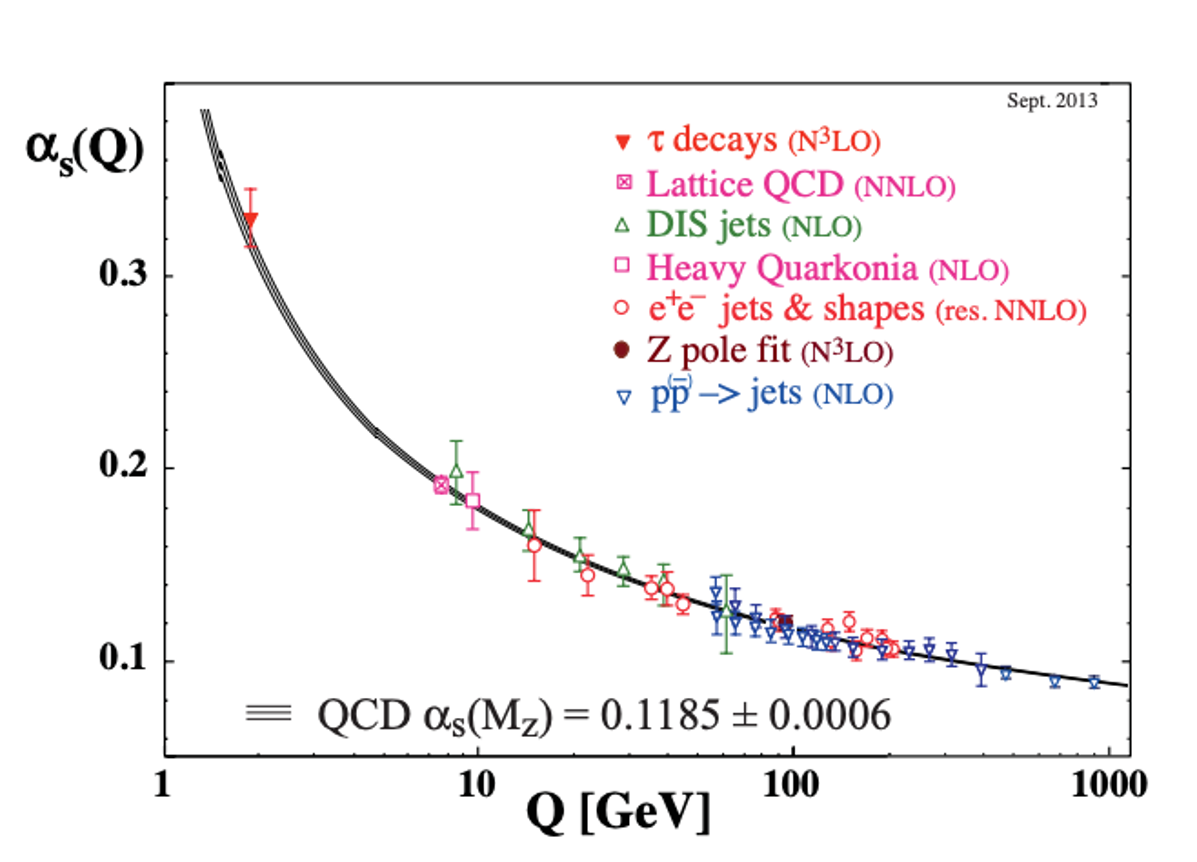
\includegraphics[width=0.7\textwidth,clip]{figures/Chapter1/Alpha_s.png}
    \end{center}
    \caption[$\alpha_s$随能量尺度$Q^2$变化的关系]{$\alpha_s$随能量尺度$Q^2$变化的关系,2014 review of paritcles}
    \label{fig:Alpha_S}
\end{figure}

渐进自由带来了几个有趣的结果。首先在大$Q^2$区间,$\alpha_s \ll 1$。这使得微扰理论在此能量尺度下仍然可以起作用。但随着$Q^2$的减小,$\alpha_s \geq 1$,从而使得微扰量子色动力学不再适用。因此其他的理论被发展出来在此区间进行量子色动力学的计算。目前比较成功的非微扰量子色动力学的计算方式为格点量子色动力学(Lattice QCD)。